
\section{The cuprate phase diagram}

The phase diagrams for the \highTc materials show a remarkable consistancy across the cuprates\footnote{This is in constrast with the recently discovered pnictide materials which show significant variations in scalings and even composition}. However this universality amongst the cuprates comes with an abundance of features which provide for some complex physical interactions and fragile intermediate `crossover' phases. The tuning parameter for the cuprate phase diagram is either electron or hole doping typically performed by elemental substitution at the crystal growth stage or by oxygen incorporation through annealing. as shown in figure~\ref{Fig:Intro:ElecHolePhaseDiagram}, the two types of doping are not symmetric with hole doping generally resulting in more robust superconductivity. For this reason the literature has largely concentrated on the hole doped preogression and as a result it is far better characterised. The doping is usually expressed as a $p$ value which represents the amount of additional holes (electrons) per Cu atom.  This thesis deals with the hole doped curpate \BSCO.
\begin{figure}[htbp]
    \begin{center}
        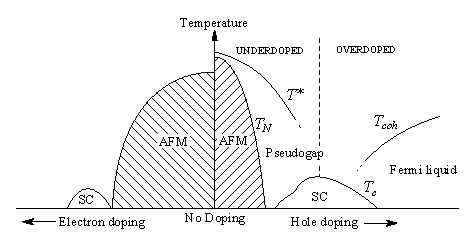
\includegraphics[scale=0.9]{Chapter-Introduction/Figures/ElecHolePhaseDiagram/ElecHolePhaseDiagram}
        \caption{A schematic phase diagram showing electron doped to the left and hole doped to the right. AFM is the antiferromagnetic Mott insulating phase, SC is the superconducting phase. $T^*$, $T_N$, $T_c$ and $T_{\textrm{coh}}$ are the temeprature scales for the pseudogap, AFM state, superconductivity and coherent Fermi liquid phases respectively}
        \label{Fig:Intro:ElecHolePhaseDiagram}
    \end{center}
\end{figure}

\subsection{Mott insulating parent compound}

Starting at the middle of figure~\ref{Fig:Intro:ElecHolePhaseDiagram}, the parent compound materials at zero doping are though to be Mott insulators i.e. the top most filled state on each lattice site contains one electron. In the conventional band picture this should be metallic since the bands are only partially filled, however when we consider a local picture of electrons, any movement of an electron to the neighbouring lattice site will cause an energetically costly double occupancy on one site and zero occupancy on another. This causes the electronic \ac{DOS} to become gapped around the Fermi surface and hence supressed conduction. This is known as the Mott insulating state.

We find that the kinetic energy term is reduced when the ordering of the sites is antiferromagnetic since for any hopping to occur at all, the spins must be antialigned to avoid double occupancy of like spins. This region dominates the low doping portion of the pahse diagram and remains antiferromagnetic until either the temperature is high enough to allow transitions from the Fermi energy to the states at the edge of the gap or the doping has introduced enough double occupancy electrons on lattice sites, which can move without the double occupancy energy cost, to overcome the insulating behaviour.

\subsection{Superconducting dome}

With increased doping, the antiferromagnetic state gives way to the superconducting dome at around $p=0.05$ which itself gives way to a Fermi liquid metallic state at a doping of around $p=0.3$. The maximum \Tc occurs at around $p=0.19$. Transitions from both the antiferromagnetic and the superconducting state are clearly second order thermodynamic with jumps in the heat capacity for example, however there are other regions in the phase diagram which are less well defined such as the pseudogap and the Fermi liquid crossover whose temeprature scale can depend on the particular probe used.

\subsection{The pseudogap}

Above the \ac{AFM} region and the superconudcting state is one of the most contraversial regions of the phase diagram is the so called pseudogap phase. This is a region which was first demonstrated in 1989, just a few years after the discovery of the cuprate materials, by \ac{NMR} measurements performed at Bell labs~\cite{Warren1989}. A noticeable fall in the susceptibility occured at a temperature significantly above \Tc which led to conclusion of possible spin pairing before the onset of bulk superconductivity\footnote{Unpaired electrons contribute to the magnetic susceptibility response, Cooper paired electrons in the singlet state have zero net spin hence the explanation as to the reduction in susceptibility}. The question arose as to what the exact relation of the pseudogap is to the superconducting state --- is it a precursor state, from which superconductivity arises or is it a competing phase? --- and from a materials development point of view, to obtain higher \Tc should we be finding ways to suppress the crossover to the pseudogap state or encourage it?

By finding where exactly the $T^*$ energy scale meets the superconducting dome, strong evidence can be found that supports one or the other scenario. However the problem lies in the type of probe used. Spectroscopic measurements such as \ac{STM} and \ac{ARPES} have found that the $T^*$ overreaches the superconducting dome entireley, meeting with the overdoped edge at $T=\unit{0}{\kelvin}$. This supports the precursor state theory where paired electrons from the pseudogap phase cross into the region where under the $T_{\textrm{coh}}$ curve which contains coherent quasiparticles. Where the two combine superconductivity arises (i.e. coherent Copper pairs).

A second scenario from bulk thermodynamic probes such as heat capcity and magnetic susceptibility measurements have shown the $T^*$ energy scale drops into the top of the superconducting dome. This support the scenario where the pseudogap is in competition with superconductivity for states near the Fermi surface. Once the pseudogap phase is suppressed, scattering from quantum fluctuations at zero temeprature leads to the formation of the superconducting phase at a \ac{QCP} similar to that found in heavy fermion materials.


% Three conflicting pictures have emerged based on the extent to which the pseudogap region overreaches the superconducting dome. 
% \begin{enumerate}
% \item $T^*$ drops into the top of the superconducting dome down to a \ac{QCP} hidden by the superconductivity. Similarly the coherence temperature does the same thing but from the overdoped side.
% \item $T^*$ overreaches the superconducting dome entirely meeting the superconducting transition at $T=\unit{0}{\kelvin}$ on the overdoped side.
% \item $T^*$ drops into the top of the superconducting dome but stops there with the energy gap due to pairing giving way to the superconudcting energy gap.
% \end{enumerate}
% 

 in many spectroscopic probes such as \ac{STM} and \ac{ARPES} the existance of an energy gap and the possibility of Cooper pairs as evidenced by Nernst measurements. However 

Figure~\ref{Fig:Intro:PhaseDiagrams} shows the phase diagram for \TODO{Give a particular example that includes electron doping} in particular that demonstrates both electron and hole doped progressions. Looking more closely at the hole doping side, which in general is where the superconductivity is more robust, we start in a Mott insulating antiferromagnetic \ac{SDW} state in the undoped parent compound, this gradually dissapates as doping is introduced along the temeprature scale, T$_N$



\section{Mott physics}

The Hubbard model takes the relatively simple and solvable tight-binding model and introduces an Anderson term which raises the energy for double occupancy by an amount $U$, known as the `Hubbard U'. This simple change deeply enriches the physics with one of the outcomes being the existance of the Mott insulating state which occurs when each lattice site is half filled with a single electron. The energy cost for an electron to hop to an adjacent site is so high that it locks the electrons in place, preventing effective conduction. Introducing holes (or electrons) allows once again hopping to take place and the eigenstates are no longer entireley localised.
